\documentclass{article}
\usepackage[utf8]{inputenc}
\usepackage{listings}
\usepackage{graphics}


\title{Concurrent and Distributed Systems
SantaWorkshopProblem}

\author{OPREA ȘTEFANIA LARISA}

\date{January 2022 CEN 3.2B}


\begin{document}

\maketitle
\newpage
\textbf{
\section{Problem statement:
Oh, Christmas joy!}}

Santa Klaus and his staff (elves and reindeer) are preparing for
another wonderful Christmas that brings joy and gifts to all children around the world.
For this homework, we had to implement a workshop for Santa that may contain factories, he has elves that creates toys and reindeer that wrap the toys into gifts.The workshop plan
has some rules that will ensure that all gifts are created in due-time and that no child is left without a present (would be such a pity).
He instructed us to tell you the following things that he has in his workshop:\\

\subsection{He has multiple toys factories:} 
- Random number of factories (between 2-5) that create toys (he does’t know how many are
needed until your factory plan is created and runs)\\
- All factories are in matrix like form (random NxN, where N is between 100-500)\\
- Each factory contains an array list with elves\\
- Every few seconds the factory will ask all its elves their position in the factory\\
- There can be no more than N/2 number of elves in a factory\\

\subsection{He has elves. Elves are really important; they create all the nice toys. Here’s what he told us about them:} 

- Elves are spawning randomly in each factory at a random place in the factory (random time\\
between 500-1000 milliseconds)\\
- When elves are spawned randomly they need to tell the factory that they are there\\
- No two elves can be on the same position\\
- Each elf works independently of any other elf\\
- Elves create gifts by:\\
a. Moving in one direction (left, right, up, down)\\
b. When they reach a wall of the factory they move in any other direction than the wall’s\\
c. Once they move they also create the gift\\
d. If an elf is surrounded by other elves and cannot move it stops for a random time
(between 10-50 milliseconds)\\
e. When the gift is created they update their factory to know what gift they created and
the factory will ask all elves to pass on the information on their location to give it to
Santa\\
f. After the elf creates a gift, he needs to rest for a short while (30 milliseconds)
*) They are really fast\\
g. Elves will work like in... forever (well, at least until December 25Th. As such they don't need to stop.\\
\subsection{He also has reindeer:}
- Reindeer await to receive gifts from the factory. Reindeer are available in the workshop\\
- They can always read from the factories the number of gifts (and which gifts), but they won’t be allowed access when elves notify the factories about new gifts or when the factory itself asks the elves about new gifts\\
- A maximum of 10 reindeer can read from a factory at a time\\
- A random time must pass between two consecutive factory readings\\
- Reindeer will put all gifts through a pipe to give to Santa\\
- Multiple reindeer at the same time put the gifts while Santa reads by itself all gifts\\
- Reindeer are known from the beginning (there are more than 8, because Santa needs backup).\\
\subsection{The main Santa’s Workshop will do the following:}

- this workshop contains all factories\\
- it creates the factories\\
- it also spawns elves and gives them a random factory to work in (remember that each elf is responsible to register himself to the factory)\\

\newpage

\section{Introduction}

 To solve this problem we had to implement different classes, so I created:\\
 -Planner(main)\\
 -Elf class\\
 -Reindeer class\\
 -Factory class\\
 -Workshop class\\
 -SantaClaus class\\
 -Gift class\\
 -GiftTransfer class\\
 
 And I did an additional task so for this one i used the class ElfRetirement class.This is the additional task I tried to implement: 1.You can retire an elf.

\section{Planner(main)}
In main we create an object of class workshop.


\section{Elf class}

In the Elf class we create elves (random time between 500-1000 milliseconds) that are spawning randomly in each factory at a random place in a specific factory from the workshop.Here we implement the moving direction for each elf and assign every elf to a factory.\\
We have a function for moving the elf can move in all directions(up.down,left,right), in this function it tries to move, as it moves the elf creates gifts, for each position moved in any direction it creates one gift and give it to the factory.When the elf hits the wall it goes in the other direction and if it has not option of moving (so its unable to move) the elf has to wait a random time (between 10-50 milliseconds).And here we call the retire elf function to the factory for it to retire the elf.

\section{Elf retirement}
After the elf creates a gift it retires, triggering another elf to be added.

\section{Reindeer class}

In the Reindeer class we give the reindeer access to the data(number of gifts and the list of gifts) from the factory, they read the data and get assigned to a factory.All the reindeer are spawned when the factories are created.While the reindeer runs, it continuously reads all the data from all the factories , then it checks if it has been assigned to a factory for transport.With the gift, it opens a communication line with the workshop via a socket. When the socket is open, the gift is sent, then the socket closes.
The loop repeats until the workshop stops working.

\section{Factory class}

Santa has multiple factories, the number of factories that it can create is a random number between 2 and 5.
The Factory class handles the elves, keeps the gifts, and notifies the workshop when they have a large enough stock of gifts. At random times, it also requests the position of all elves.\\
Here we have the function that gives the size of the factory that is a square matrix NxN, where N is between 100-500 and the number of gifts per factory 25-100.The run() function of the factory, at first, continuously checks the number of gifts currently in the possession of the factory. When a certain threshold is passed, the factory will announce to the workshop that there are gifts ready to be delivered.Workshop will further announce the reindeer which will come and pick up the gifts.\\
If there are gifts that need to be transported, if it is done and if we have enough gifts its stops elves and it announces the workshop.
It adds elves given from the workshop to the factory grid and here we print the position where the elf was created and number of the elf that was spawned.The elves move in the factory and give gifts to the factory and here we print the factory where the gift was created.

\section{Gift class}

Each factory and elves has a unique assigned code/serial, which is used only for debugging and testing purposes. 

\section{GiftTransfer class}

Used to transfer gifts to Santa.

\section{SantaClaus class}

 Here Santa puts the gifts gained in his sack, he doesn't need rest.
 \newpage
 
\section{Workshop class}

Workshop class is the center of the simulation.
In this class we create the factories a random number between 2 and 5 and the reindeer also a random number between 8 and 10.
Run() tries to add elves while there are factories running.
As the assignment specifies that the workshop can only process only one gift at a time, only one thread is required for the  communication on the server side. After the gift
is received, the socket is closed and the gift is added in the gifts vector.
The workshop also acts as a middle man between the factory and the reindeer. As its been specified that the reindeer can be found at the workshop, I supposed that the workshop dispatches the reindeer to retrieve the gifts from the factories, but only when the factory requires a transport. The factories, when they consider that they have a large enough number of gifts, notify the factory that they are ready for a shipment. The
factory dispatches all the available elves to that factory.\\
When a factory finishes it‘s job, the workshop is notified. In turn, when
all the factories are done, all the elves and reindeer stop working.

\section{Observations}
The extra task that I tried to implement, it works, but a elf is spawned, it moves and automatically create a gift, then it stops and retire, I couldn't do the task to retire a elf after more moves.

\section{Testing}
The start of the test:
\begin{center}

  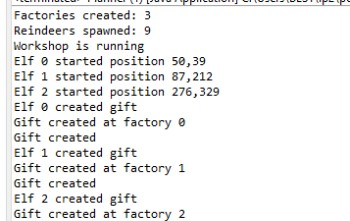
\includegraphics{test.JPG}

\end{center}
\newpage
The end of the simulation:
\begin{center}

  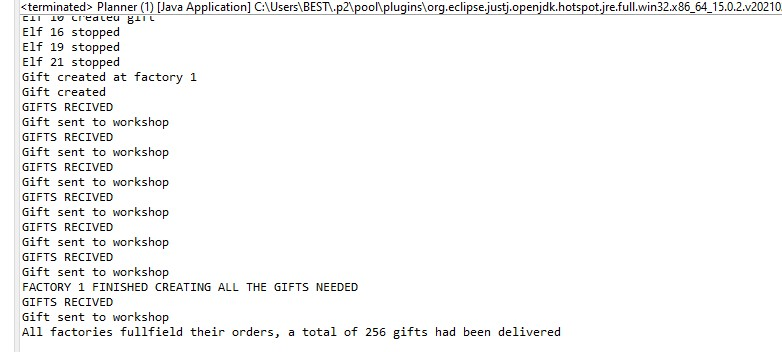
\includegraphics{test1.JPG}

\end{center}
\end{document}
